\documentclass{beamer}

\usepackage{beamerthemesplit}
\usepackage{mathrsfs}  
\usepackage{amsmath}

\usetheme{boxes} 
\setbeamertemplate{items}[default] 
\setbeamertemplate{blocks}[rounded]
\setbeamertemplate{navigation symbols}{} 
 
% Math macros
\newcommand{\cD}{{\mathcal D}}
\newcommand{\cF}{{\mathcal F}}
\newcommand{\todo}[1]{{\color{red}{TO DO: \sc #1}}}

\newcommand{\reals}{\mathbb{R}}
\newcommand{\integers}{\mathbb{Z}}
\newcommand{\naturals}{\mathbb{N}}
\newcommand{\rationals}{\mathbb{Q}}

\newcommand{\ind}[1]{1{\{#1\}}} % Indicator function
\newcommand{\pr}{\mathbb{P}} % Generic probability
\newcommand{\ex}{\mathbb{E}} % Generic expectation
\newcommand{\var}{\textrm{Var}}
\newcommand{\cov}{\textrm{Cov}}

\newcommand{\normal}{N} % for normal distribution (can probably skip this)
\newcommand{\eps}{\varepsilon}
\newcommand\independent{\protect\mathpalette{\protect\independenT}{\perp}}
\def\independenT#1#2{\mathrel{\rlap{$#1#2$}\mkern2mu{#1#2}}}

\newcommand{\convd}{\stackrel{d}{\longrightarrow}} % convergence in distribution/law/measure
\newcommand{\convp}{\stackrel{P}{\longrightarrow}} % convergence in probability
\newcommand{\convas}{\stackrel{\textrm{a.s.}}{\longrightarrow}} % convergence almost surely

\newcommand{\eqd}{\stackrel{d}{=}} % equal in distribution/law/measure
\newcommand{\argmax}{\arg\!\max}
\newcommand{\argmin}{\arg\!\min}
 \newcommand{\bit}{\begin{itemize}}
 \newcommand{\eit}{\end{itemize}}
 
 
%%%%%%%%%%%%%%%%%%%%%%%%%%%%%%%%%%%%%%%%%%%%%

\title{A review of ``On the Failure of the Bootstrap for Matching Estimators'' (Abadie and Imbens; 2008)}
\author{Andrew Do, Kellie Ottoboni, Simon Walter}
\date{April 8, 2016}

\begin{document}

\frame{\titlepage}

\section[Outline]{}
\frame{\tableofcontents}

\section{Introduction}

\frame{
\frametitle{Problem}

\bit
\item Matching is sometimes done to control for pretreatment covariates in observational studies
\item Matching estimators are nonlinear functions of the data and do not follow any nice known distribution
\item \textbf{Problem:} how do you find standard errors for matching estimators?
\item Two common ways: asymptotic approximations and resampling methods
\eit
}

\frame
{
  \frametitle{The bootstrap}
  Sample with replacement from the observed data, pretending it is the population, to approximate the distribution of the statistic

\begin{figure}  
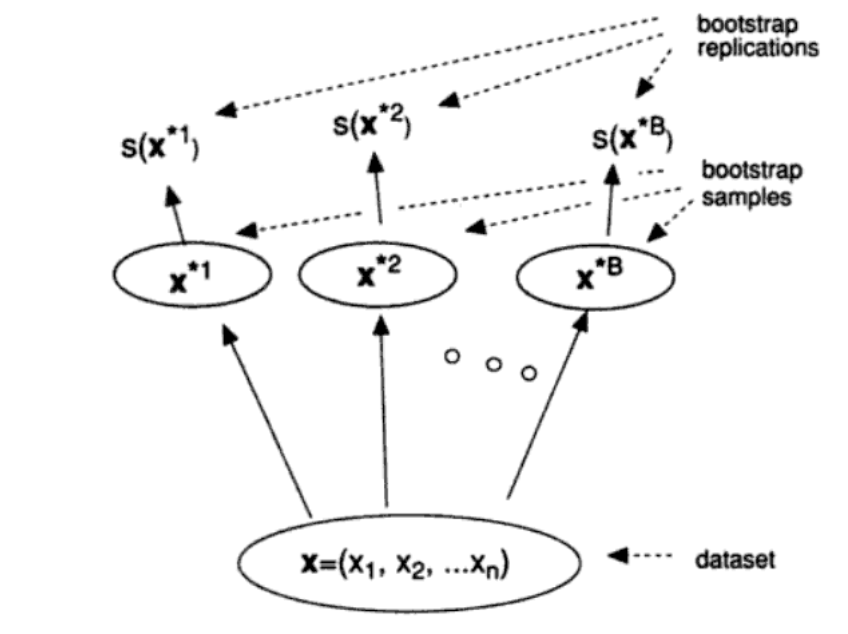
\includegraphics[width = 0.7\textwidth]{fig/scheme.png}
\caption{Taken from Efron and Tibshirani (1993)}
\end{figure}
}





\frame{
\frametitle{On the failure of the bootstrap}

The bootstrap estimate of the variance of the matching estimator $\hat{\tau}$ is given by
$$\hat{V}^B = \frac{1}{B} \sum_{b=1}^B \left( \hat{\tau}_b - \hat{\tau} \right)^2$$

\textbf{Abadie and Imbens show that $\hat{V}^B$ is not generally valid for matching estimators.} \\
\vspace{10pt}
They focus on the case of one-to-one matching on a single continuous covariate.
}


\section{Abadie and Imbens (2008)}

\subsection{Notation and Assumptions}

\frame{
\frametitle{Notation and Assumptions}
\begin{itemize}
\item Suppose we have a random sample of $N_0$ units from the control population and a random sample of $N_1$ units from the treated population, with $N = N_0 + N_1$
\item Each unit has a pair of potential outcomes, $Y_i(0)$ and $Y_i(1)$, under the control and active treatments
\item Let $W_i$ indicate treatment: we observe $Y_i = W_i Y_i(1) + (1-W_i) Y_i(0)$
\item In addition to the outcome, we observe a (scalar) covariate $X_i$ for each individual
\end{itemize}
We're interested in the \textbf{average treatment effect for the treated} (ATT):

$$\tau = \ex(Y_i(1) - Y_i(0) \mid W_i = 1)$$
}


\frame{
\frametitle{Notation and Assumptions}

We make the usual assumptions for matching:

\begin{itemize}
\item Unconfoundedness: For almost all $x$,
$$(Y_i(0), Y_i(1)) \independent W_i \mid X_i = x \text{  almost surely}$$
\item Overlap: For some $0 < c < 1$ and almost all $x$,
$$c \leq \pr(W_i = 1 \mid X_i = x) \leq 1-c$$
\end{itemize}
}



\frame{
\frametitle{Notation and Assumptions}
$D_i$ is the distance between the covariate values for observation $i$ and the closest control group match:

$$D_i = \min_{j = 1, \dots, N: W_j = 0} \left\Vert X_i - X_j \right\Vert$$

\vspace{20pt}
$\mathcal{J}(i)$ is the set of closest matches for treated unit $i$. 

\begin{displaymath}
   \mathcal{J}(i) = \left\{
     \begin{array}{lr}
       \{ j \in \{1, \dots, N\} : W_j = 0, \left\Vert X_i - X_j \right\Vert = D_i \} & \text{ if  } W_i = 1\\
       \emptyset & \text{ if  } W_i = 0
     \end{array}
   \right.
\end{displaymath} 

If $X$ is continuous, this set will consist of one unit with probability 1. In bootstrap samples, units may appear more than once.
}


\frame{
\frametitle{Notation and Assumptions}
Estimate the counterfactual for each treated unit as:

$$\hat{Y}_i(0) = \frac{1}{\# \mathcal{J}(i)} \sum_{j \in \mathcal{J}(i)} Y_i$$

The matching estimator of $\tau$ is then

$$\hat{\tau} = \frac{1}{N_1} \sum_{i : W_i = 1} \left(Y_i - \hat{Y}_i(0)\right)$$
}




\frame{
\frametitle{Notation and Assumptions}
An alternative way of writing the estimator is

$$\hat{\tau} = \frac{1}{N_1} \sum_{i=1}^N (W_i - (1-W_i)K_i) Y_i$$

where $K_i$ is the weighted number of times that unit $i$ is used as a match:

\begin{displaymath}
   K_i = \left\{
     \begin{array}{lr}
      0 & \text{ if  } W_i = 1\\
      \sum_{j: W_j=1} \ind{i \in \mathcal{J}(j)} \frac{1}{\#\mathcal{J}(j)} & \text{ if  } W_i = 0
     \end{array}
   \right.
\end{displaymath} 
}



\subsection{The Bootstrap}



\frame{
\frametitle{Bootstrap}
\bit
\item We obtain a \textbf{bootstrap sample} $Z_b$ by taking a random sample with replacement from $Z= (X, W, Y)$. 
\item Let $\hat{\tau}_b = t(Z_b)$ be the matching statistic computed on bootstrap sample $b$.
\item The bootstrap variance of $\hat{\tau}$ is the variance of $\hat{\tau}_b$ conditional on the original data $Z$:

$$V^{B} = \ex\left[ (\hat{\tau}_b - \hat{\tau})^2 \mid Z\right]$$

\item We estimate it by generating $B$ bootstrap samples from $Z$ and taking the following average:

$$\hat{V}^B = \frac{1}{B} \sum_{b=1}^B \left( \hat{\tau}_b - \hat{\tau} \right)^2$$
\eit
}


\frame{
\frametitle{Bootstrap}
\bit
\item The bootstrap works for linear statistics that are  asymptotically normal
\item For nonlinear statistics, the bootstrap requires additional smoothness conditions.
\item We will address each of these points in detail later.
%\todo{cite?}
\item Earlier work also by Abadie and Imbens show that $\hat{\tau}$ is asymptotically normal and provides a consistent estimate of the variance.
\item Why does the bootstrap fail here? 
\eit


}


\frame{
\frametitle{Bootstrap}
\textbf{Issue:} the bootstrap fails to replicate the distribution of $K_i$, even in large samples.
\vspace{10pt}


Example:
\begin{itemize}
\item Suppose the ratio $N_1/N_0$ is small (i.e. there are many more controls than treated)
\item In the original sample, few controls are used as a match more than once
\item In bootstrap samples, treated units may appear multiple times, creating situations where $\pr(K_{b,i} > 1) > \pr(K_i > 1)$ 
%\todo{is this technically correct? is there a better way to put this?}
%I think this is correct -SW
\end{itemize}
}


\section{Simulations} % can change the subsection headings...

\subsection{Example 1} % Andrew results

\subsection{Example 2} % Kellie results


\frame{
\frametitle{Effect of covariate distributions}

\bit
\item Potential outcomes $Y(1)$ and $Y(0)$ defined as before
\item Treatment assigned at random with $\frac{N_1}{N_0} = \alpha = 2$ fixed
\item Change the covariate distributions: $X_i \sim N(0, 1)$ if $W_i = 1$ and $X_i \sim N(\mu, 1)$ if $W_i = 0$.
\item We vary $\mu$ from $0$ to $5$
%\item \todo{this slide is ugly}
\eit
}

\frame{
\frametitle{Results}
\begin{figure}[htbp]
\begin{center}
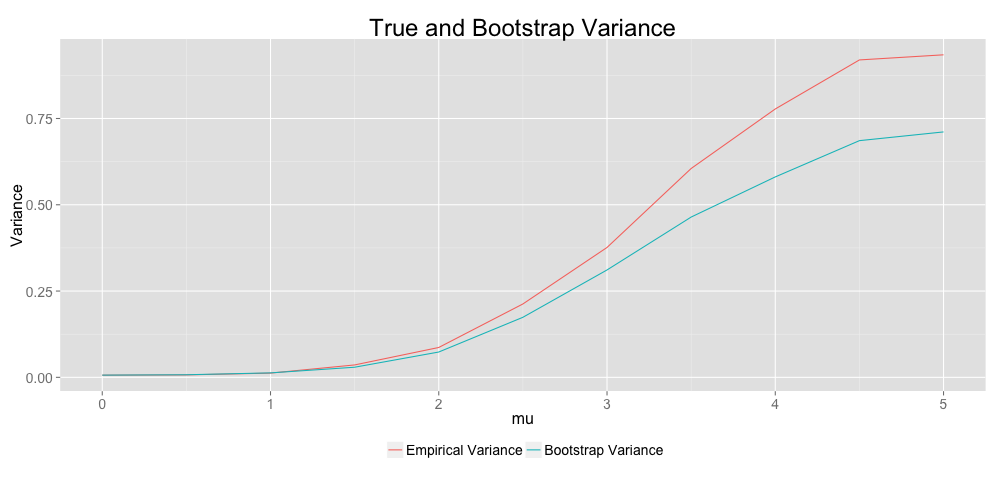
\includegraphics[width = 0.85\textwidth]{fig/KellieSimulationBias.png}
\end{center}
\end{figure}

The bootstrap tends to underestimate the variance of $\hat{\tau}$.  The bias increases as the distance $\mu$ between treatment and control groups increases.
}


\frame{
\frametitle{Results}
\begin{figure}[htbp]
\begin{center}
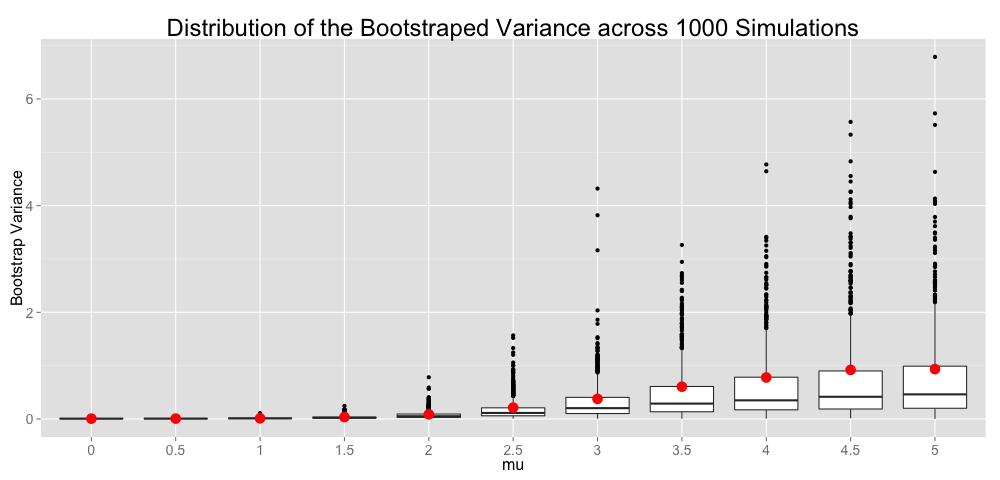
\includegraphics[width = 0.9\textwidth]{fig/KellieSimulationDistr.png}
\end{center}
\end{figure}

Red points indicate the observed variance of the test statistic.  The distribution of bootstrap variances has a long right tail. The skew worsens as $\mu$ grows.

}
\section{A theoretical view}
\frame{
\frametitle{Previous work on the bootstrap}
\bit
\item The bootstrap has been with us in its modern form since 1977.
\item The procedure works in a very wide variety of situations but there are several famous examples where the bootstrap fails:
\bit
\item $X_i \overset{iid}{\sim} \mathscr{U}(0,\theta)$ and $\hat{\theta} = X_{(n)}$
\item $X_i \overset{iid}{\sim} \mathscr{N}(\mu, 1)$ where $\mu \in [0, \infty)$ and $\hat{\mu}= \max(0, \bar{X})$; 
\item $X_i \overset{iid}\sim \mathscr{N}(\mu, 1)$ and $\hat{\mu}= \begin{cases} 
b \bar{X}_n \textrm{  if $ |\bar{X}_n| < n^{-1/4}$} \\
\bar{X}_n \textrm{  if $ |\bar{X}_n| \geq n^{-1/4}$}
\end{cases}$  $b \in (0,1)$
\eit

\item There are some big theorems guaranteeing the consistency of the bootstrap in general situations.
\eit
}

\frame{
\frametitle{When does the bootstrap work?}

%\item There is a widespread but imperfect and outdated intuition that states that Efron's bootstrap consistently estimates the distribution of the statistic  if and only if the statistic is asymptotically normal. 
Cs\"{o}rg\H{o} and Mason (1989) prove a result regular linear statistics summarized by Mammen 1992.
\begin{theorem}
If $\theta(F) = \frac{1}{n} \sum_{i-1}^n h_n(X_i)$ for some arbitrary function $h_n$ then the bootstrap works in the sense that $$d_\infty\big[\mathscr{L}(\theta(\hat{F})-\hat{t}_n), \mathscr{L}(\theta(F)-t_n)\big] \underset{p}{\rightarrow} 0$$ if and only if there exists $\sigma_n$ and $t_n$ such that $$d_\infty\big[\mathscr{L}(\theta(F)-t_n), N(0, \sigma_n^2)\big]\underset{p}{\rightarrow} 0$$
Where $\hat{t}_n$ is some function of our sample (typically the statistic itself) and $t_n = \mathbb{E}(\hat{t}_n)$
\end{theorem}

}
\frame{
The next theorem is from Politis, Romano and Wolf (1999).
A statistic is Fr\'echet differentiable if $$\theta(G) = \theta(F) + L_F(G-F) + o(\Vert G - F\Vert)$$ as $\Vert G - F \Vert \rightarrow 0$ for some linear functional $L_F$.
\begin{theorem}
Let $\mathscr{F}$ be the class of all distributions with finite support. Assume that $F$ is drawn from $\mathscr{F}$ and the statistic $\theta(\cdot)$ is Frechet differentiable at $F$  and $L_F$ satisfies a certain condition. Then $\theta(F)$ is asymptotically normal and the bootstrap works in the sense of the previous theorem.\end{theorem}

 High level intuition for this theorem is that we want to have $\hat{F} \rightarrow F \Rightarrow \theta(\hat{F}) \rightarrow \theta(F)$. This is very similar to the usual definition of continuity from analysis.

}
\frame{
\frametitle{Is there an if and only if result for smooth functionals}
\bit
\item There are cases of statistics that are not Fr\`{e}chet differentiable for which the bootstrap works (eg the sample median) but ...
\item According to Mammen (1992), van Zwet (1989) suggests smoothness is not only sufficient but necessary. 
\item van Zwet (1989) was a seminar given at a conference in 1989 in Germany and unfortunately I can find no record of it.
\item Cursory comments in Mammen (1992) suggest the argument is by way of the Hoeffding decomposition theorem, but I don't currently understand this theorem or the proof strategy.
\eit
}
\frame{
\frametitle{Placing Abadie and Imbens in the literature}
\bit
\item Some of this theoretical work on the bootstrap is not well known by practitioners, and it may be that early versions of Abadie and Imbens (2008) were written without detailed knowledge of this work.

\item Arguably, the results of Abadie and Imbens are not surprising and  not entirely novel to statisticians familiar with the theoretical work of the 1980s.
\item The statistic of the matching estimator investigated is not smooth because if a treated $X_i$ falls exactly at the midpoint between two control $X_j$, $X_k$ the statistic changes discontinuously if we shift $X_i$ infinitesimally closer to one  of $X_j$ or $X_k$.
\item But the paper is very valuable because it highlights for practitioners one of the (many) limitations of the vanilla bootstrap. 
%\item For example in the Beran's (1982) example it is not hard to show this is violated:
%\begin{align*}
%\theta(X_1, \ldots, X_n) \Longrightarrow
%N\left[\mu, \frac{1}{n} \var(X))\right] \textrm{\quad   if $E(X) \neq 0$} \\
%\theta(X_1, \ldots, X_n) \Longrightarrow N\left[\mu, \frac{b^2}{n} \var(X)\right] \textrm{\quad   if $E(X) = 0$}
%\end{align*}

\eit
}
\frame{
\frametitle{Contribution to theoretical understanding of the bootstrap}
\bit
\item In a longer version of their paper Abadie and Imbens suggest this is the first case for which the bootstrap is inconsistent for a statistic that is asymptotically normal and $\sqrt{n}$-consistent.
\item But this is not quite true. An example we have already discussed due to  Beran (1982) also exhibits bootstrap failure and is asymptotically normal and asymptotically unbiased:

$$\theta(X_1, \ldots, X_n) = \begin{cases} 
b \bar{X}_n \textrm{  if $ |\bar{X}_n| < n^{-1/4}$} \\
\bar{X}_n \textrm{  if $ |\bar{X}_n| \geq n^{-1/4}$}
\end{cases}$$
Although in this case bootstrap  failure only occurs on a set of Lebesgue measure zero
\item The proof of this fact is not easy.
\eit
}

%\frame{
%\frametitle{Contribution to theoretical understanding of the bootstrap}
%
%\bit
%\item In the final version of the paper,  Abadie and Imbens emphasize the unusualness of an example for which the bootstrap is inconsistent for a statistic that is asymptotically normal, $\sqrt{n}$-consistent and \underline{asymptotically unbiased}.
%
%\item This is not the first  example either because Beran's 1982 example is also asymptotically unbiased. 
%
%\eit
%}


\frame{
\frametitle{An example of bootstrap inconsistency for an unbiased statistic}
\bit
\item It is also not too difficult to construct other simpler examples where the bootstrap fails on a parameter set with positive measure that are unbiased for finite samples and not just asymptotically; although they seem  not to have previously appeared in the literature.

\item We give one here: suppose $X_i$ are drawn iid from  $\{\normal(\mu, 1)\}_{\mu \in \mathbb{R}}$ .
\item Our estimate for $\mu$ is $$\theta(\hat{F}) = \theta(X_1, \ldots, X_n) = \bar{X} + \#\{(i,j) : X_i = X_j, i \neq j \}$$
\item Under the true sampling distribution the second summand is almost surely zero.
\item But under the bootstrap distribution the second summand is at least one with probability $1 - n!/n^n$
\eit
}
\frame{
\frametitle{An example of bootstrap inconsistency for an unbiased statistic}\bit
\item The previous example is unnatural and unlikely arise in practice.
\item But it does not seem hard to extend this to cases of practical interest involving ties.
\item For example the critical value of Wilcoxon rank-sum and signed rank tests might be approximated using the bootstrap when ties are present in the data.
\item Alternatively an analyst might try to approximate the distribution of the Kolmogorov-Smirnov test statistic using the bootstrap. 
\eit
}




\frame{
\frametitle{Should we follow Abadie and Imbens recommendation?}
\bit
\item Main conclusion is  only their prior work based on asymptotic normality or subsampling  have formal justification.
\item Subsampling is seldom used in practice because it is sensitive to the choice of subsample size, and it is typically difficult to find the optimal subsample size from data.
\item Using asymptotic normality is not  satisfying either because it is only `first order' correct; on the other hand the bootstrap is often `second order' correct. 
\item What does this mean ... ?
\eit
}

\frame{
\bit
\item For many statistics of interest we can form Edgeworth expansions of the distribution function:
$$ \pr(\sqrt{n}(\hat{\theta} - \theta_0)/\sigma \leq x) = \Phi(x) + n^{-1/2} p_1(x) \phi(x) + \ldots$$
\item The $p_j(x)$ are polynomials with coefficients determined by low order moments of the statistic.
\item The bootstrap distribution has a similar expansion:
$$ \pr^*(\sqrt{n}(\hat{\theta}^* - \hat{\theta})/\hat{\sigma} \leq x) = \Phi(x) + n^{-1/2} \hat{p}_1(x) \phi(x) + \ldots$$
\item Here the $\hat{p}_j(x)$  are $p_j(x)$ with population moments substituted for their empirical counterparts.
\item Bootstrap is second order correct if $$n^{-1/2} \hat{p}_1(x) \phi(x) = n^{-1/2} p_1(x) \phi(x) + o(n^{-1/2})$$
\eit

}
\section{Rescuing the bootstrap}
\frame{
\frametitle{Can we rescue Efron's bootstrap for matching estimators?}
\bit
\item If we can make our statistic asymptotically smooth in an appropriate sense then we should be OK.

\item A natural way to do this is to let the number of matches, $m$, increase with $N_0$.
\item Tentative empirical results suggest the consistency of the bootstrap depends on the rate at which $m$ grows. 
\bit
\item $m  \asymp  \sqrt{N_0}$ yields intervals with incorrect coverage.
\item $m \asymp \log(N_0)$ yields intervals with asymptotically correct coverage.
\eit
\item But in both cases the 2006 result of Abadie and Imbens using asymptotic normality seems to fail. 
\eit 
}

\frame{
\frametitle{Simulation results for fixing the bootstrap}
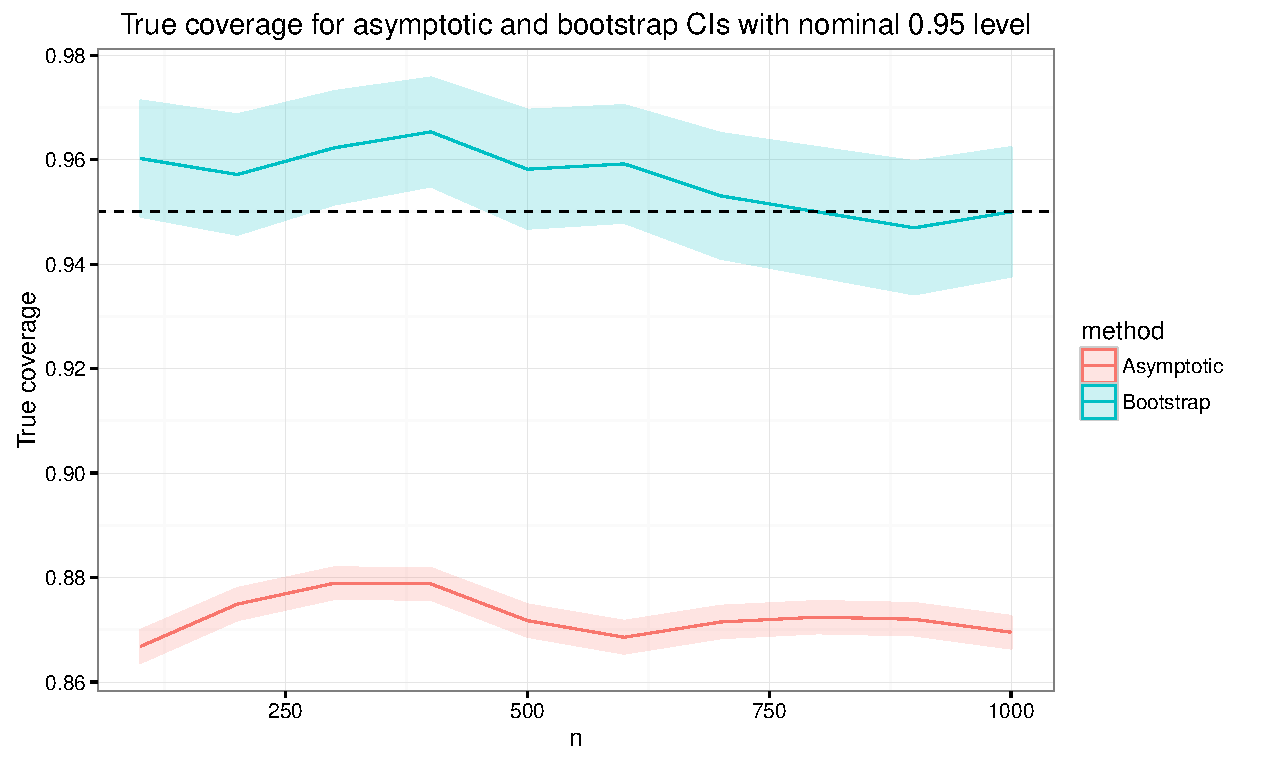
\includegraphics[width = 4in]{fig/SWIncreasingMatches.PDF}


}



\subsection{Example 3} % Simon results


\frame{
\frametitle{Conclusions}
\bit
\item Efron's bootstrap will not work for this kind of matching estimator with a single match on one covariate when the distribution of Y(0) is not degenerate.
\item We can save the bootstrap by making the estimator smoother asymptotically or by subsampling.
\item Although we did not discuss it there might be other fixes too including the $m$-out-of-$n$ bootstrap and the wild bootstrap.
\item There is also relatively recent work that suggests that Efron's bootstrap may be preferable even when it is not consistent because it outperforms other (possibly consistent) methods in finite samples.
\eit
}



\end{document}
